\head{Алгоритмы на строках}
Сегодня нас ждёт тема, которой не было в первой версии книги. Идея добавления этой главы возникла из-за поездки автора книги в Сириус. Поэтому сегодня мы пройдём базовые алгоритмы на строках: хэширование, z-функцию и префикс-функцию. Стоит отметить, что алгоритмов на строках достаточно много, но в этой главе будут рассмотрены только самые простые.


\subhead{Хэширование}
Пусть перед нами стоит такая задача: дано $m$ строк: $a_1,\ a_2,\ \ldots,\ a_m$, каждая из которых имеет длину $n$. Требуется проверить все пары строк на равенство.

Понятно, что эта задача решается за \O{m^2 \cdot n} простым перебором всех пар строк и их посимвольным сравнением. Но всё же интересно, можно ли решать эту задачу быстрее? Оказывается, что да: можно сравнивать две строки за \O{1} с помощью \term{хэшей}, но при этом такое сравнение может иногда выполняться не точно. Но давайте разберёмся со всем по порядку.

Хэшем называется преобразование набора данных произвольной длины в данные какой-то фиксированной длины. При этом. судя по происхождению от слова \term{hash} (переводится как \term{превращать в фарш} или \term{мешанина}), исходный набор данных восстановить нельзя. Поскольку длина выходного хэша фиксирована, то неизбежны \term{коллизии} — то есть совпадение хэшей для разных входных данных. Но поскольку вероятность коллизий мала, особенно при правильном выборе хэш-функции, то они используются на практике как в практических задачах, так и в олимпиадном программировании.

Оказывается, что в качестве хэша в олимпиадных задачах очень удобно использовать функцию вида: $h = s_1 + s_2 \cdot P + s_3 \cdot P^2 + \ldots + s_n \cdot P^{n - 1}$, где $s$ — исходная строка, $h$ — результирующий хэш, а $P$ — постоянное число. При этом логично выбирать $P$ простым, и большим, чем размер используемого алфавита (символы, которые потенциально могут встретиться в строке). Если бы числовые типы данных были бы произвольного размера и всегда бы быстро сравнивались, то таких хэши получались бы разными для разных строк. Но поскольку встроенные длинные типы данных есть не во всех языках, а их сравнение всё равно выполняется долго, то считая эту сумму по какому-нибудь модулю, мы увеличиваем шанс коллизий, но при этом ускоряем алгоритм. На практике в C++ брать по модулю не обязательно, ведь встроенные типы данных сами это делают при переполнении, поэтому можно просто считать эту сумму, ни о чём не думая :)


% ababcaba
% 0 0 2 0 0 3 0 1
\subhead{Z-функция}
Теперь, когда мы научились проверять две строки на равенство, хочет научиться и более сложным операциям, например вычислять на сколько две строки похожи. Но две строки — это слишком много, поэтому давайте мы их склеим через какой-то разделитель и будем смотреть на сколько конец строки похож на её начало.

Более формальное определение \term{z-функции}: $z_i$ — это количество символов, начиная с позиции $i$, совпадающих с началом строки. При этом $z_1$ фактически не даёт полезной информации, поэтому можно считать, что $z_1 = 0$ или $z_1 = n$, где $n$ — длина строки. Эту функцию легко посчитать за \O{n^2}, ведь для каждой позиции можно перебирать все идущие после неё символы. Но такая сложность нас не устраивает, ведь можно написать более быстрый алгоритм.

Для этого будем поддерживать наибольший уже просмотренный отрезок $[l; r]$, совпадающий с началом строки $[0; r - l]$. Тогда при вычислении $z_i$ могут возникнуть всего две ситуации:

\begin{itemize}
    \item Если $i$ не лежит в отрезке $[l; r]$, то воспользоваться предыдущей информацией не получится. поэтому будем вычислять тривиальным алгоритмом.
    \item Если же $i$ в $[l; r]$, тогда мы знаем, что часть строки $[i; r]$ такая же, что и $i - l, r - l$. Поэтому за первое приближение можно взять $z_i = z_{i - l}$, но нужно учесть, что такое $z_i$ не выходит за границы $[l; r]$ (потому что в $z_{i - l}$ случайно мог быть очень большим). После же такого приближения тривиальным алгоритмом можно вычислить $z_i$ точно. 
\end{itemize}

А после вычисления $z_i$ можно обновить $[l; r]$ на $[i; i + z_i - 1]$, если у нового отрезка правый конец правее старого. Для большего понимания описанного выше алгоритма, хочется привести код, его реализующий:

\cpp{str-1}{14}

Теперь перейдём к оценке сложности алгоритм. Кажется, что мы недалеко ушли от тривиального решения, ведь мы добавили всего пару проверок. Но на самом деле этот алгоритм работает за \O{n}, потому что всегда при вычислении нового $z_i$ используется как можно больше старых данных, поэтому все новые вычисления производятся только после позиции $r$, ну а границы движутся только вправо, откуда и получаем линейную сложность.

% 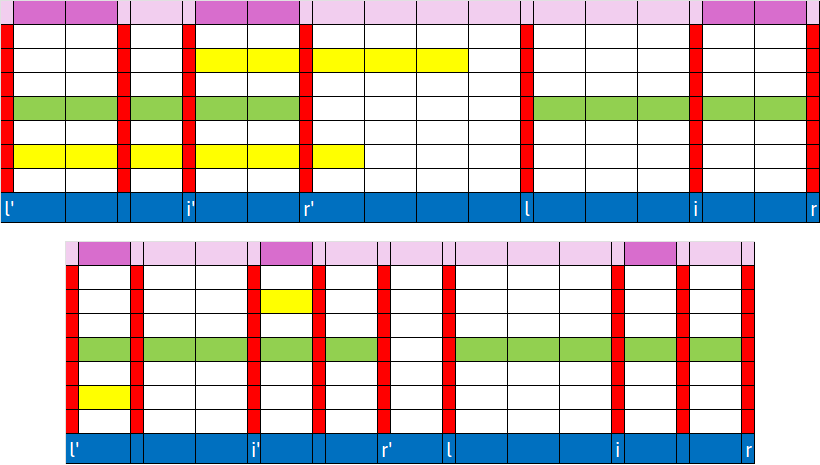
\includegraphics[scale=0.73]{img/z_function.png}


% ababcaba
% 0 0 1 2 0 1 2 3
\subhead{Префикс-функция}
\term{Префикс-функция} это ещё один способ проверить на сколько часть строки похожа на её начало. А именно, $p_I$ — это самое большое количество символов такое, что часть $[i - p_i + 1, i]$ совпадает с началом строки.

Зачем же нам ещё одна функция очень похожая на предыдущую? А вот оказывается, что обе функции бывает запомнить сложно, но одну через другую вспомнить проще. К тому же для сложных алгоритмов может понадобиться какая-то конкретная из этих двух функция.

Теперь прейдём к её работе. По определению префикс-функции при вычислении $p_i$ мы знаем, что часть строки $[0; p_{i - 1})$ совпадает с $(i - 1 - p_{i - 1}; i - 1]$. Тогда, если так оказалось, что $s_i = s_{p_{i - 1}}$, то нашли самый большой подходящий отрезок. Иначе же нам стоит уменьшить отрезок префиксной-функции на один, причём мы вполне можем перейти в начало строки, ведь оно аналогично её концу.

Для наглядности приведём код и этого алгоритма:

\cpp{str-1}{12}

Оказывается, что и этот алгоритм выполняется за \O{n} (ведь иначе о нём было бы странно рассказывать :) ). Такая сложность получается из-за того, что от позиции к позиции значение префикс-функции или уменьшается, или увеличивает не больше, чем на один. А раз так, то всего таких увеличений (и соответственно уменьшений) не больше, чем количество символов в строке, а поскольку каждое увеличение и уменьшение делается быстро, то итоговая сложность линейная.


\subhead{Применение этих алгоритмов}
Разных задач, конечно же, много, но всё же часть из них стоит кратко упомянуть, ведь они решаются через пройденные в этой главе алгоритмы. 

\textbf{Проверка на палиндромность}. Пусть у нас для одной строки поступает много запросов, для которых требуется проверить, является ли фрагмент строки $[l; r]$ палиндромом. Здесь нам на помощь придут хэши, ведь, по сути, требуется проверять, равна ли строка её развороту. А значит посчитаем хэш для обычной строки и хэш для развёрнутой. Тогда при аккуратной работе с индексами, мы можем получить хэш одного участка строки и слева, и справа, и если эти хэши окажутся равны, то значит фрагмент строки является палиндромом.

\textbf{Сжатие строки}. Предположим. что какую-то короткую строку записали несколько (возможно не целое) количество раз и дали нам полученную длинную строку. Требуется понять, какой могла быть короткая строка и из всех этих вариантов выбрать с самой короткой строкой. Вот оказывается, что ответом будет строка $[0; i)$, где $i$ — первый индекс, для которого выполняется равенство $i + z_i = n$.

\textbf{Поиск подстроки в строке}. Пусть нам требуется найти какой-то образец длины $n$ в тексте и вывести все позиции, где этот образец начинается. Тогда, как уже говорилось выше, давайте сделаем одну строку, в начале которой будет образец, потом разделитель (этот разделитель не должен встречаться в строках), а в конце уже сам текст. Тогда понятно, что все $i$, для которых выполняется $z_i = n$ являются началами вхождений образца. Для префикс-функции же, имеем $p_i = n$ для концов образцов.
